\section{Manual Installation}
\label{appendix:appendix_a}

We are pleased to offer you all the necessary tools required to effortlessly set up the CAD infrastructure.
Managing the installation of Python and NPM packages is something you need not worry about,
as we have already created comprehensive images that encompass all the essential packages,
ensuring a seamless execution process. \\

It's important to note that the tools needed for the installation are
primarily focused on project building and remain independent of the services created.
Although our example uses Fedora Linux 38 as the operating system,
rest assured that all the tools used in this platform are cross-platform compatible,
guaranteeing smooth execution on other operating systems as well. \\


Here is the list of tools needed for the installation:

\begin{itemize}
  \item Git
  \item Docker or Podman
  \item docker-compose
  \item cURL
\end{itemize}

Before proceeding, please make sure you have all the required tools listed above.
Next, you'll need to become a superuser, and you can do that with the following command:

\begin{Verbatim}[fontsize=\scriptsize]
$ sudo su
\end{Verbatim}

If you opt for Docker, execute the following command to initiate the installation process:

\begin{Verbatim}[fontsize=\scriptsize]
$ curl https://raw.githubusercontent.com/wilberquito/melanoma.thesis/main/MAKE.sh | bash
\end{Verbatim}

If you prefer Podman,
you will first need to install the podman docker package to enable Podman to work harmoniously with Docker commands:

\begin{Verbatim}[fontsize=\scriptsize]
$ sudo dnf install -y podman-docker
\end{Verbatim}

Afterward, you can utilize the MAKE.sh script to build the architecture:

\begin{Verbatim}[fontsize=\scriptsize]
$ curl https://raw.githubusercontent.com/wilberquito/melanoma.thesis/main/MAKE.sh | bash
\end{Verbatim}

To confirm that the CAD infrastructure services are operational,
you can locate the two containers using the following command:

\begin{Verbatim}[fontsize=\scriptsize]
$ docker ps
\end{Verbatim}

You should see the two containers listed as shown in the image below:

\begin{figure}[H]
\centering
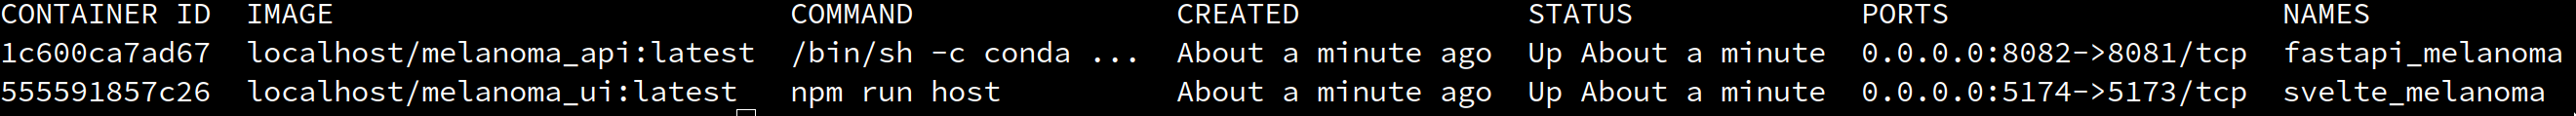
\includegraphics[width=\textwidth]{imatges/appendices/services.png}
\caption[Container CAD Services]{\textit{Container CAD Services.}}
{\label{fig:polling-layer}}
\end{figure}

The API is accessible through port 8082. To view the documentation, simply open any web browser and enter the following URL:

\begin{Verbatim}[fontsize=\scriptsize]
http://127.0.0.1:8082/docs
\end{Verbatim}

Similarly, to access the CAD UI, you can use port 5174. Just open your web browser and enter the following URL:

\begin{Verbatim}[fontsize=\scriptsize]
http://127.0.0.1:5174
\end{Verbatim}

Rest assured that with these tools and guidelines,
you'll have a smooth and successful installation of the CAD infrastructure.
